% Slides for 2024-04-08
\begin{frame}{Team Changes}
    Thank you to Adrian Zugehar

    Welcome Charlie Kushlevsky (FW)
\end{frame}
\begin{frame}{Current Focus}
    \centering
    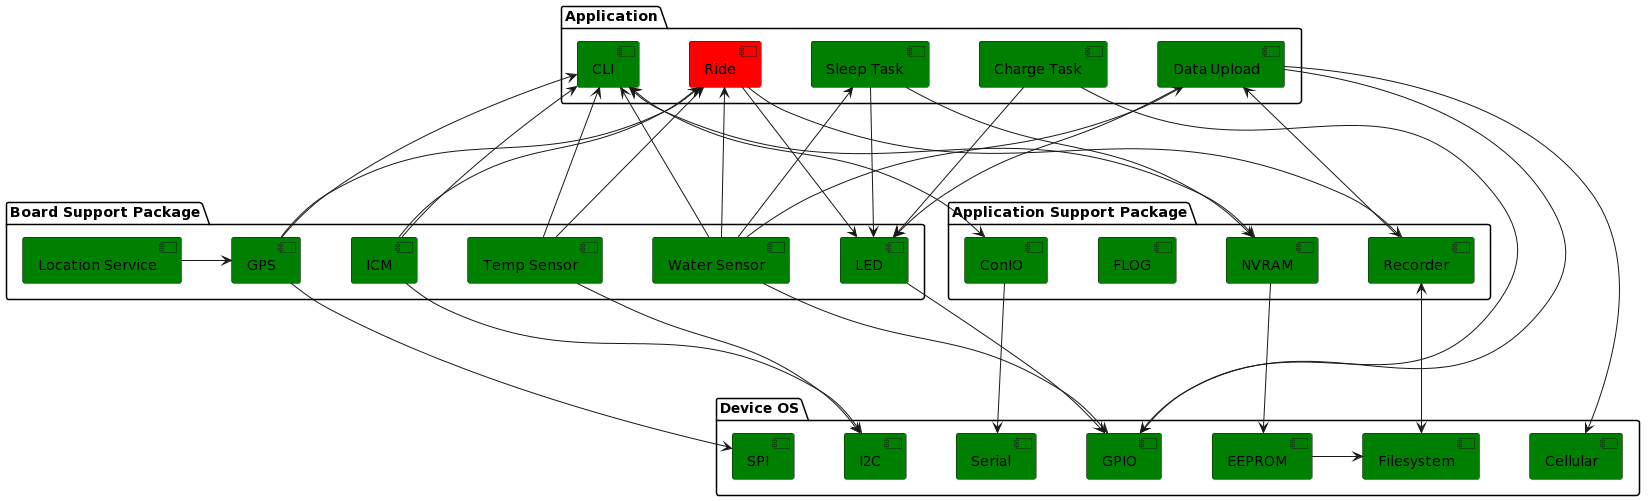
\includegraphics[height=0.7\textheight,width=\textwidth,keepaspectratio]{images/sf_service_diag.png}
\end{frame}
\begin{frame}{Planned Recruiting}
    MechE/Mfg Engineer
    \begin{itemize}
        \item CNC Machining
        \item Composites
    \end{itemize}
\end{frame}
\begin{frame}{Proposed Spin-off Project}
    OpenOceanSampler
    \begin{itemize}
        \item STM32 based
        \item GPS, INS, wet/dry, pressure, temperature
        \item Expandable platform
    \end{itemize}
\end{frame}
% To create a slide, use the following:
% \begin{frame}{TITLE}
%     BODY
% \end{frame}

% To create a slide with a bullet list, use the following:
% \begin{frame}{TITLE}
%     \begin{itemize}
%         \item ITEM 1
%         \item ITEM 2
%     \end{itemize}    
% \end{frame}

% To create a slide with numbered list, use the following:
% \begin{frame}{TITLE}
%     \begin{enumerate}
%         \item ITEM 1
%         \item ITEM 2
%     \end{enumerate}
% \end{frame}

% To create a slide with a graphic:
% 1. Add the graphic to this folder (named picture.png)
% 2. Use the following:
% \begin{frame}{TITLE}
%     \centering
%     \includegraphics[height=0.7\textheight,width=0.7\textwidth,keepaspectratio]{picture.png}
% \end{frame}

% To create a slide with two columns, use the following:
% \begin{frame}{TITLE}
%     \begin{columns}
%         \begin{column}{0.5\textwidth}
%             COLUMN 1 BODY
%         \end{column}
%         \begin{column}{0.5\textwidth}
%             COLUMN 2 BODY
%         \end{column}
%     \end{columns}
% \end{frame}
